% SPDX-License-Identifier: MIT
% Copyright (c) 2017-2020 Forschungszentrum Juelich GmbH
% This code is licensed under MIT license (see the LICENSE file for details)
%
\documentclass[
t, % align text inside frame to t=top, b=bottom, c=center
10pt, % 8pt, 9pt, 10pt, 11pt, 12pt, 14pt, 17pt, 20pt available as text font
aspectratio=169, % select your aspect ratio 4:3=43, 16:9=169, 16:10=1610
ngerman,
english,
%handout,
]{beamer}
\usetheme{Juelich}

\usepackage{babel}
\usepackage[utf8]{inputenc}
\usepackage{verbatim}

\usepackage{hyperref}
\usepackage{physics}

\usepackage{listings}
\lstset{basicstyle=\ttfamily,breaklines=true}

\newcommand{\Ciso}{$^{13}$C~}
\DeclareMathOperator{\Reals}{\mathbb{R}}
\newcommand{\deriv}[2]{\frac{\mathrm{d}#1}{\mathrm{d}#2}}

\newcommand{\templateversion}{18.10}
\newcommand{\tutorialversion}{18.10}

\title{Improving Sampling Efficiency in \Ciso MFA}
\subtitle{Master's Thesis Outline}
\author{Richard D. Paul}
%\institute[My Institute]{}
\date{\today}
\titlegraphic{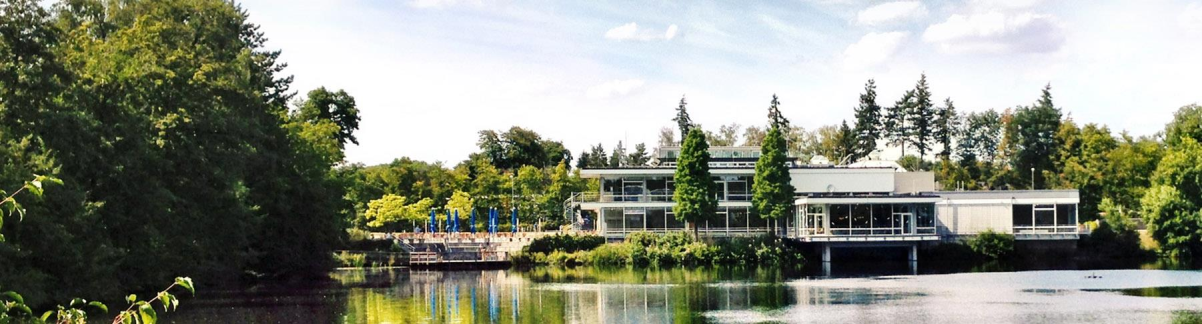
\includegraphics[width=\paperwidth]{placeholder}}

\begin{document}
\maketitle

%\begin{frame}
%    \frametitle{Metabolic Networks \& Stoichiometric Modelling}
%    \[
%	\Stoi = \begin{matrix} &
%	    {
%		\setlength\arraycolsep{8pt}
%		\begin{matrix} 
%		    
%		    u & v & w & x & y & z 
%		\end{matrix}
%	    }\\[2mm]
%	    \begin{matrix} A \\ B \\ C
%	    \end{matrix} &
%	    \begin{pmatrix}
%		-1 & & -1 & 1 & & \\ 
%		1 & -1 &  & & -1 & \\ 
%		& 1 & 1 & & & -1 
%	    \end{pmatrix}
%	    \\ \\[2mm]
%	\end{matrix}
%    \]
%    Let $\nu_i$ be the reaction rate of reaction $i$, then $\displaystyle \fracd{t} A = \nu_x - \nu_u - \nu_w$
%    \[
%	\implies \fracd{t} X = \Stoi \nu 
%    \]
%    with $X = (A, B, C)^\top$
%\end{frame}
%
%\begin{frame}
%    \frametitle{Metabolic Networks \& Stoichiometric Modelling}
%    Steady-state condition (homeostasis)
%    \[
%	\fracd{t} X = \Stoi \nu = 0 \implies \nu \in \ker(\Stoi)
%    \]
%\end{frame}

\begin{frame}[c]
    \frametitle{Roadmap}
    \begin{itemize}
	\item Experimentally assess optimal acceptance rates for model problems. Do theoretical results hold?
	\item How do non-identifiable dimensions affect the optimal acceptance rate and convergence?
	\item Combine Adaptive Metropolis with polytope samplers
	\item Is Adaptive Metropolis able to approximate optimal acceptances rates? 
	\item Does Adaptive Metropolis work with non-identifiable dimensions?
	\item What other approaches exist there? Active subspaces \cite{Constantine_2016}
    \end{itemize}
\end{frame}

\begin{frame}[c]
    \frametitle{Roadmap}
    \begin{itemize}
	\item Experimentally assess optimal acceptance rates for model problems. Do theoretical results hold?
        {\color{lgray}
	\item How do non-identifiable dimensions affect the optimal acceptance rate and convergence?
	\item Combine Adaptive Metropolis with polytope samplers
	\item Is Adaptive Metropolis able to approximate optimal acceptances rates? 
	\item Does Adaptive Metropolis work with non-identifiable dimensions?
	\item What other approaches exist there? Active subspaces \cite{Constantine_2016}
    }
    \end{itemize}
\end{frame}

\begin{frame}[c]
    \frametitle{Optimal acceptance rates}
    \begin{itemize}
        \item Performance measures:
        \begin{itemize}
            \item Effective Sample Size (ESS): \[
                    N_{eff} = \frac{N}{1 + \tau}, \quad \tau \dots \text{ autocorrelation time}
                \]
            \item Expected Squared Jump Distance (ESJD): \[
                    \mathrm{ESJD} = \frac{1}{N-1} \sum_{i=1}^{N-1} \| \theta_n - \theta_{n+1} \|_2^2
                \]
            \item Upper bound on Expected Squared Jump Distance per second (ESJD/s): \begin{align*}
                \mathrm{ESJD/s} = \frac{\mathrm{ESJD}}{t_\alpha r_\alpha + t_d},
                    & \quad t_\alpha \dots \text{ time per simulation}, \quad r_\alpha \dots \text{ acceptance rate}, \\
                    & \quad t_d \dots \text{ time per draw}
            \end{align*}
        \end{itemize}
    \end{itemize}
\end{frame}

\begin{frame}[c]
    \frametitle{Optimal acceptance rates}
    \begin{itemize}
        \item 4 chains where run until they hit convergence ($\widehat{R} < 1.05$) or maximal number of samples was exceeded
        \begin{itemize}
            \item $\widehat{R}$ can be computed incrementally
        \end{itemize}
    \end{itemize}
\end{frame}

\begin{frame}[t]
    \frametitle{Optimal acceptance rates}
    \begin{itemize}
    \item {\color{orange} Orange } upper bound on the ESJD/s
    \end{itemize}
    \centering
    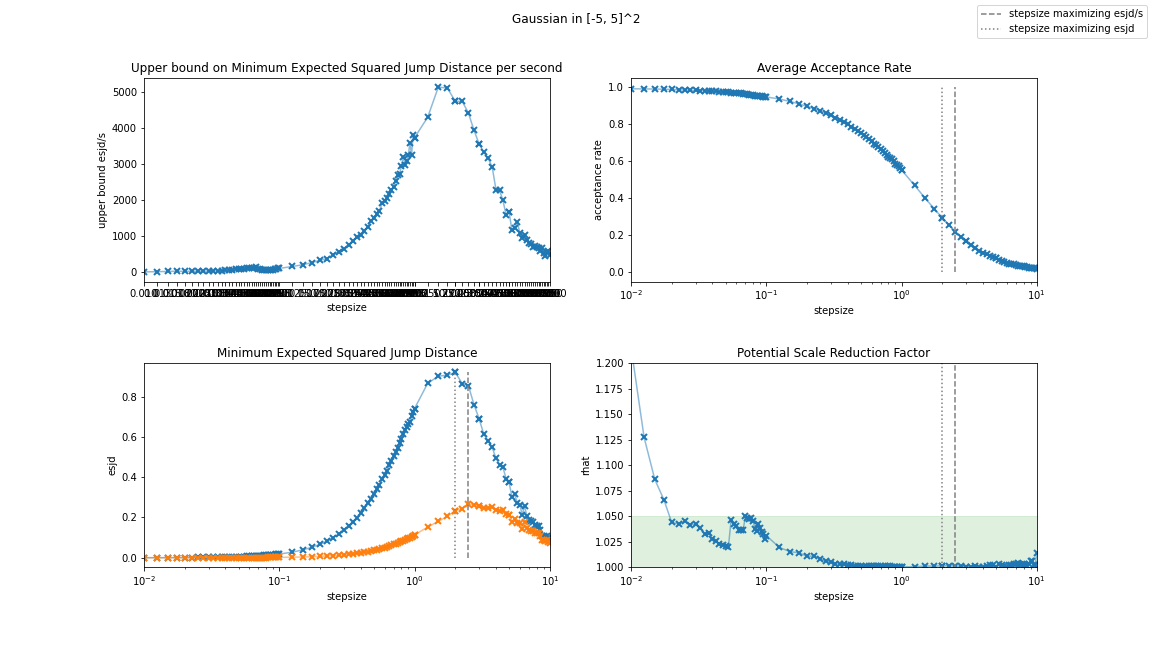
\includegraphics[width=0.7\textwidth]{imgs/bound-5-dim-2-Gaussian-results.png}
\end{frame}

\begin{frame}[t]
    \frametitle{Optimal acceptance rates}
    \begin{itemize}
    \item {\color{orange} Orange } upper bound on the ESJD/s
    \end{itemize}
    \centering
    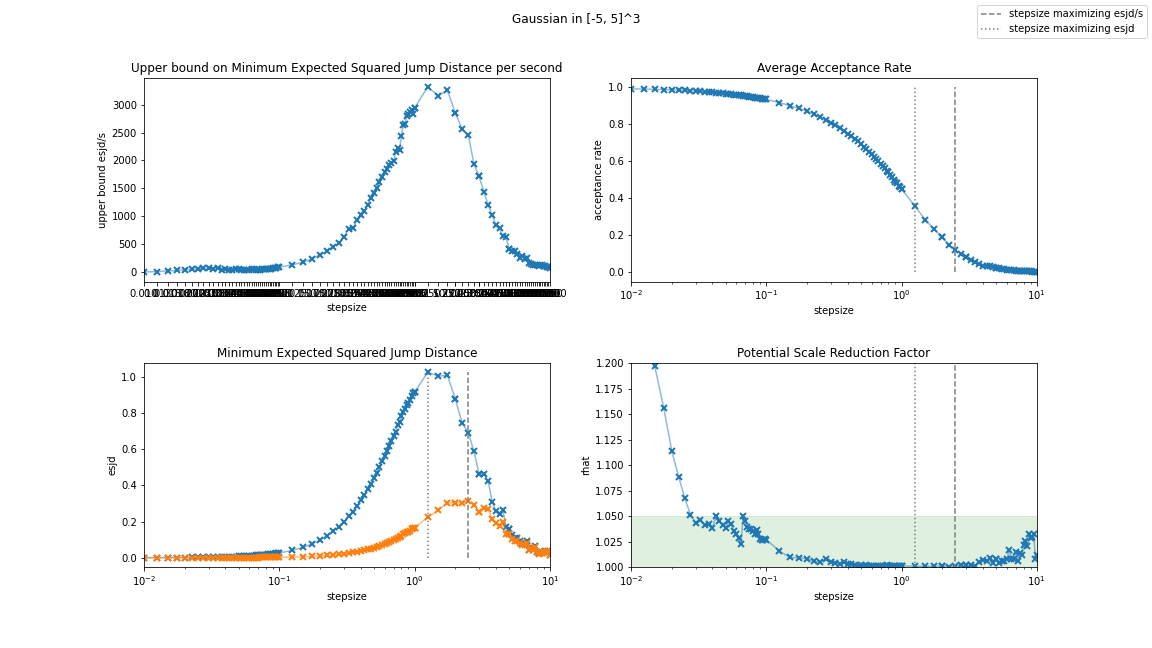
\includegraphics[width=0.7\textwidth]{imgs/bound-5-dim-3-Gaussian-results.png}
\end{frame}

\begin{frame}[t]
    \frametitle{Optimal acceptance rates}
    \begin{itemize}
    \item {\color{orange} Orange } upper bound on the ESJD/s
    \end{itemize}
    \centering
    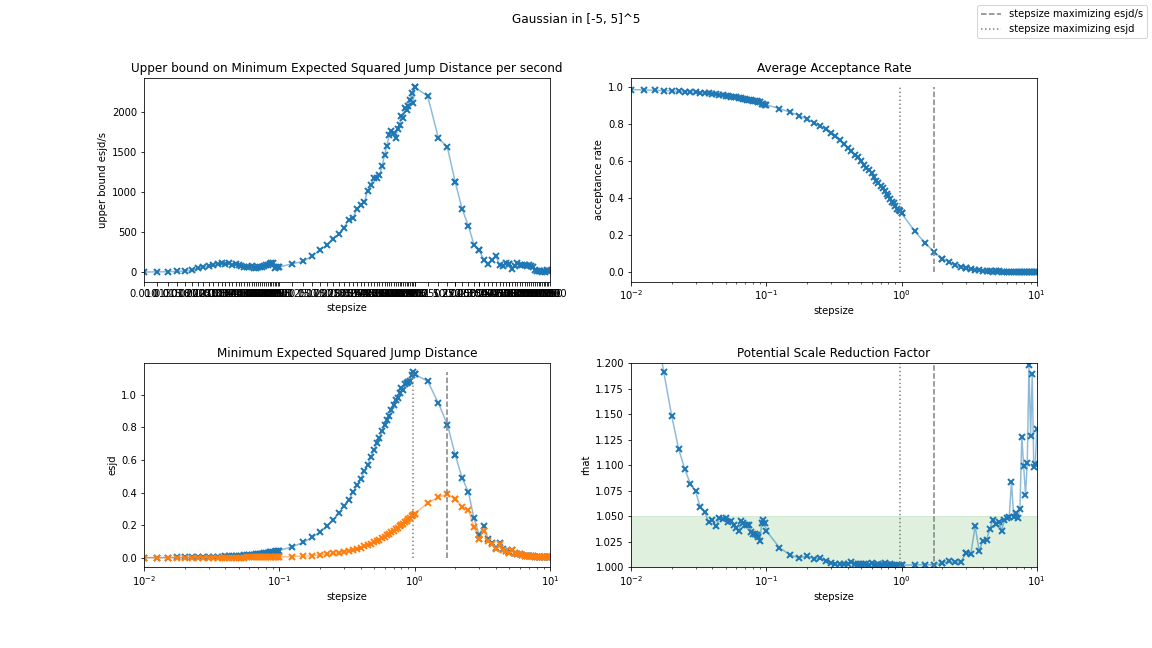
\includegraphics[width=0.7\textwidth]{imgs/bound-5-dim-5-Gaussian-results.png}
\end{frame}

\begin{frame}[t]
    \frametitle{Optimal acceptance rates}
    \begin{itemize}
    \item {\color{orange} Orange } upper bound on the ESJD/s
    \end{itemize}
    \centering
    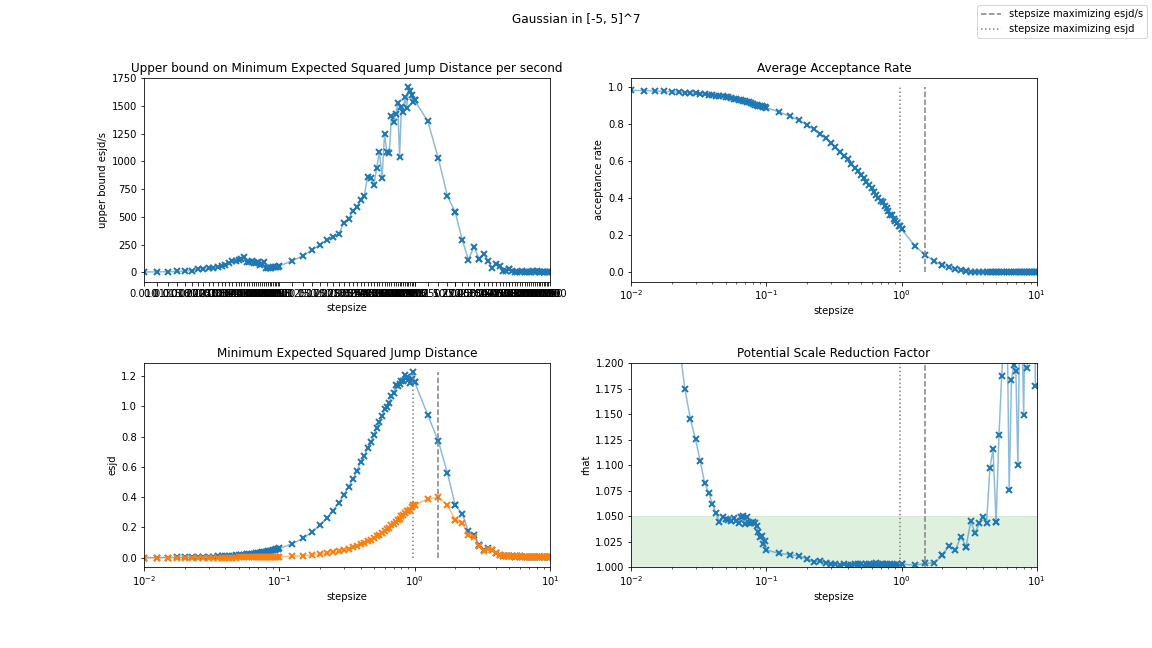
\includegraphics[width=0.7\textwidth]{imgs/bound-5-dim-7-Gaussian-results.png}
\end{frame}

\begin{frame}[t]
    \frametitle{Optimal acceptance rates}
    \begin{itemize}
        \item {\color{orange} Orange } upper bound on the ESJD/s
    \end{itemize}
    \centering
    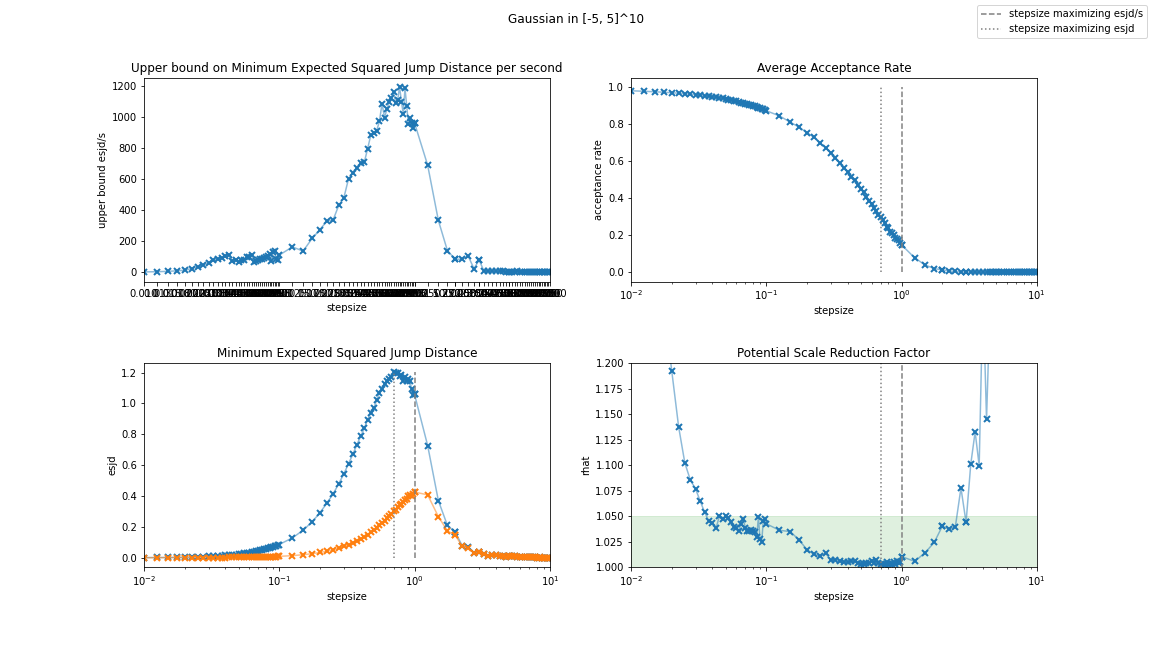
\includegraphics[width=0.7\textwidth]{imgs/bound-5-dim-10-Gaussian-results.png}
\end{frame}

\begin{frame}[t]
    \frametitle{Optimal acceptance rates}
    \begin{itemize}
    \item {\color{orange} Orange } upper bound on the ESJD/s
    \end{itemize}
    \centering
    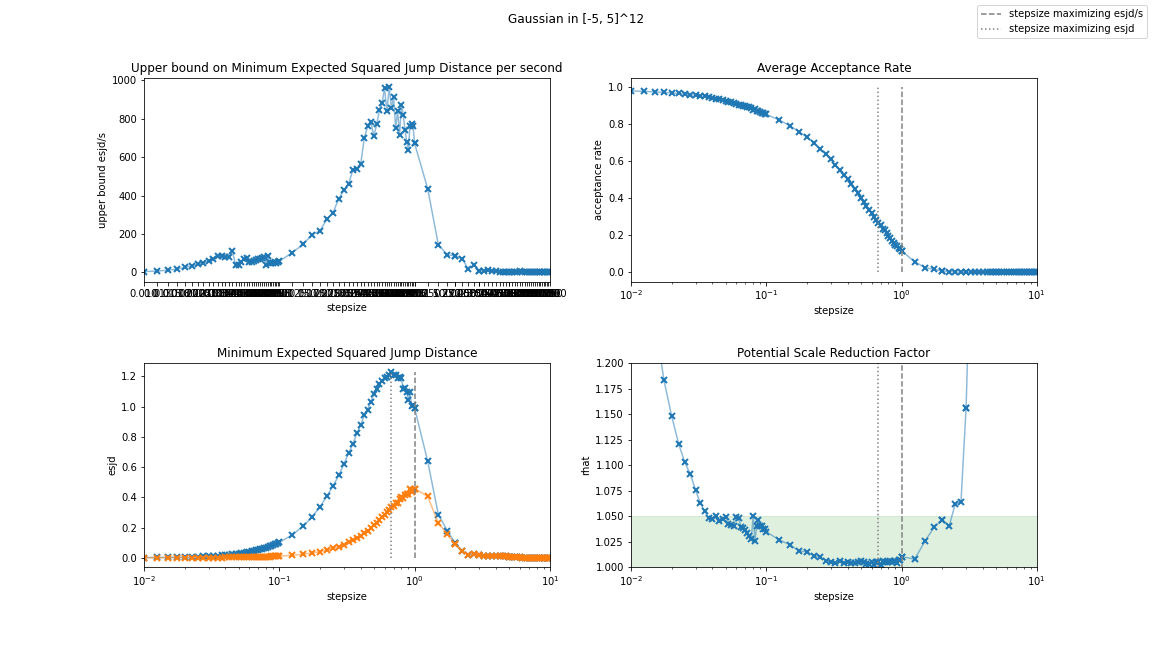
\includegraphics[width=0.7\textwidth]{imgs/bound-5-dim-12-Gaussian-results.png}
\end{frame}

\begin{frame}[t]
    \frametitle{Optimal acceptance rates}
    \begin{itemize}
    \item {\color{orange} Orange } upper bound on the ESJD/s
    \end{itemize}
    \centering
    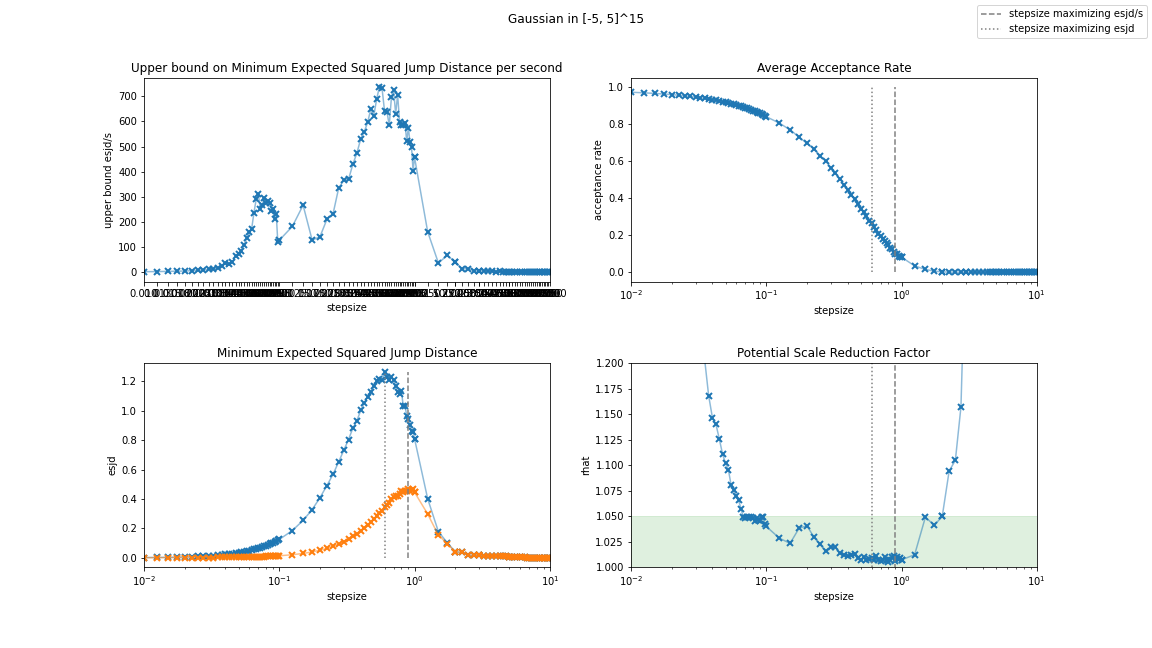
\includegraphics[width=0.7\textwidth]{imgs/bound-5-dim-15-Gaussian-results.png}
\end{frame}

\begin{frame}[t]
    \frametitle{Optimal acceptance rates}
    \begin{itemize}
    \item {\color{orange} Orange } upper bound on the ESJD/s
    \end{itemize}
    \centering
    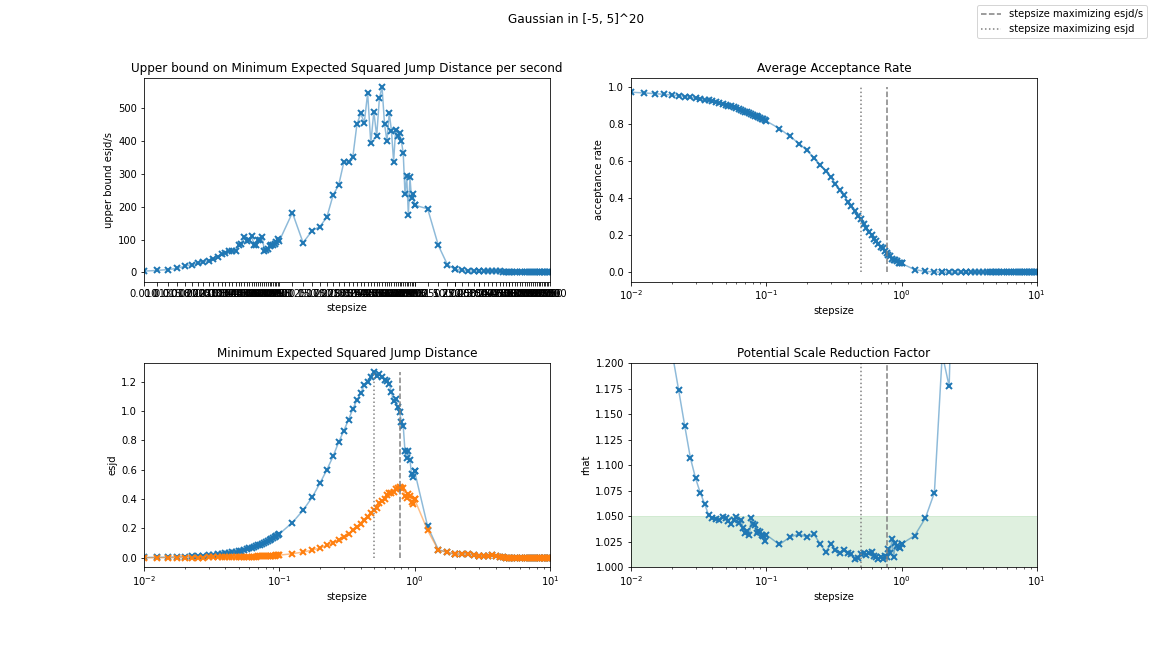
\includegraphics[width=0.7\textwidth]{imgs/bound-5-dim-20-Gaussian-results.png}
\end{frame}

\begin{frame}[t]
    \frametitle{Optimal acceptance rates}
    \begin{itemize}
    \item {\color{orange} Orange } upper bound on the ESJD/s
    \end{itemize}
    \centering
    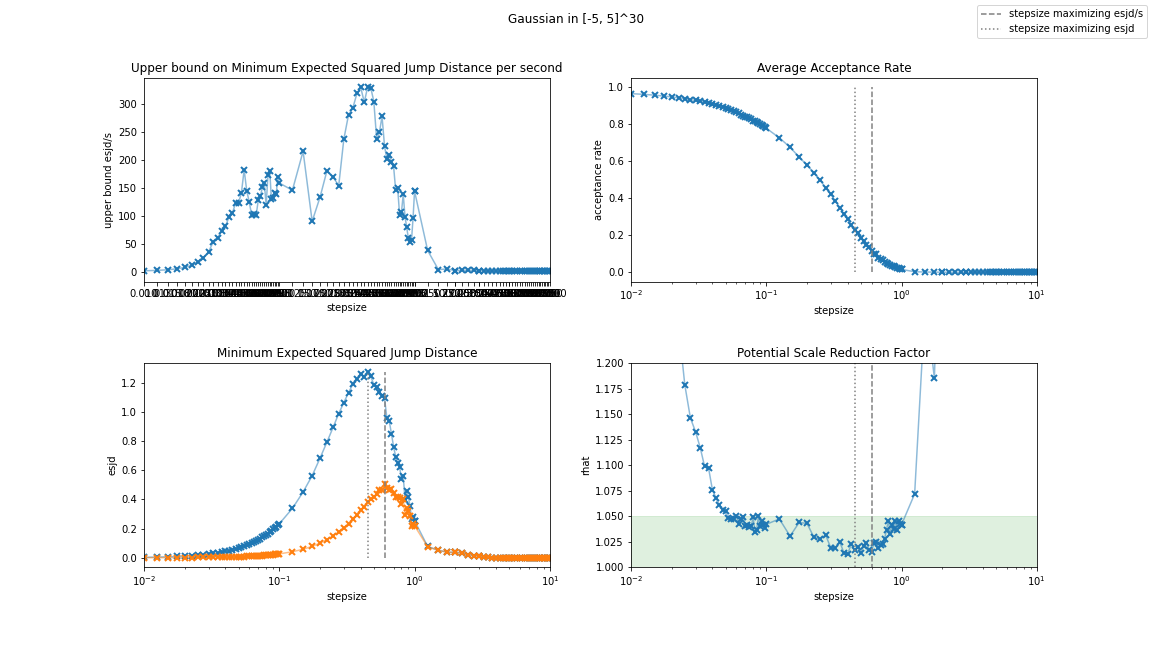
\includegraphics[width=0.7\textwidth]{imgs/bound-5-dim-30-Gaussian-results.png}
\end{frame}

\begin{frame}[t]
    \frametitle{Optimal acceptance rates}
    \begin{itemize}
    \item {\color{orange} Orange } upper bound on the ESJD/s
    \end{itemize}
    \centering
    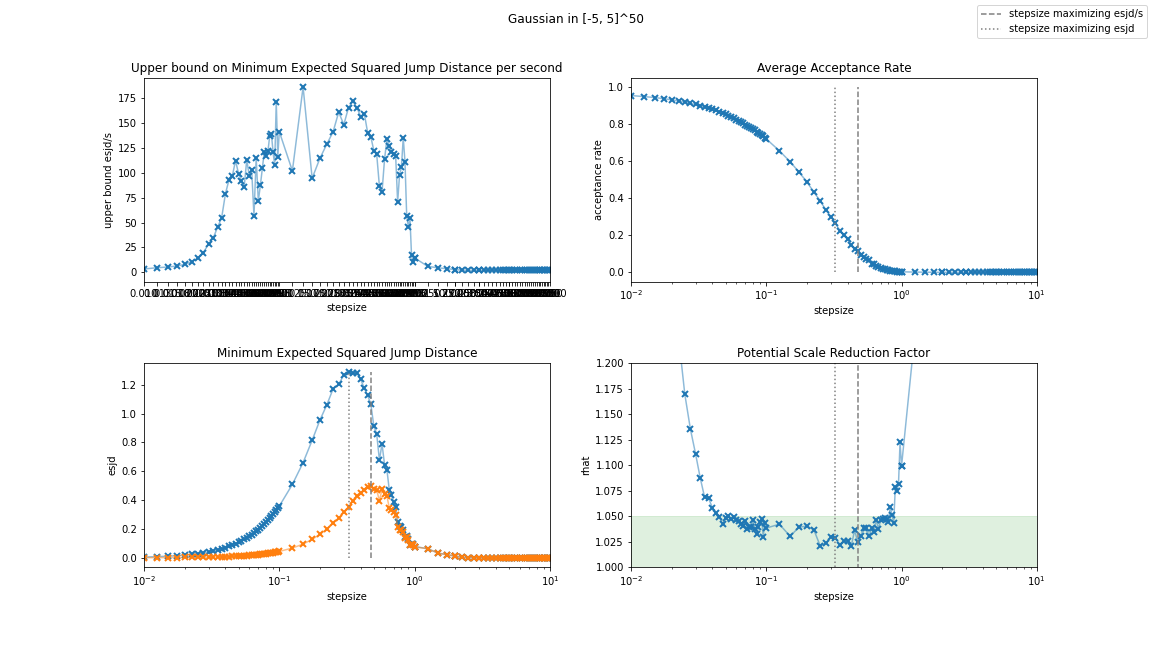
\includegraphics[width=0.7\textwidth]{imgs/bound-5-dim-50-Gaussian-results.png}
\end{frame}

\begin{frame}[t]
    \frametitle{Optimal acceptance rates}
    \begin{itemize}
    \item {\color{orange} Orange } upper bound on the ESJD/s
    \end{itemize}
    \centering
    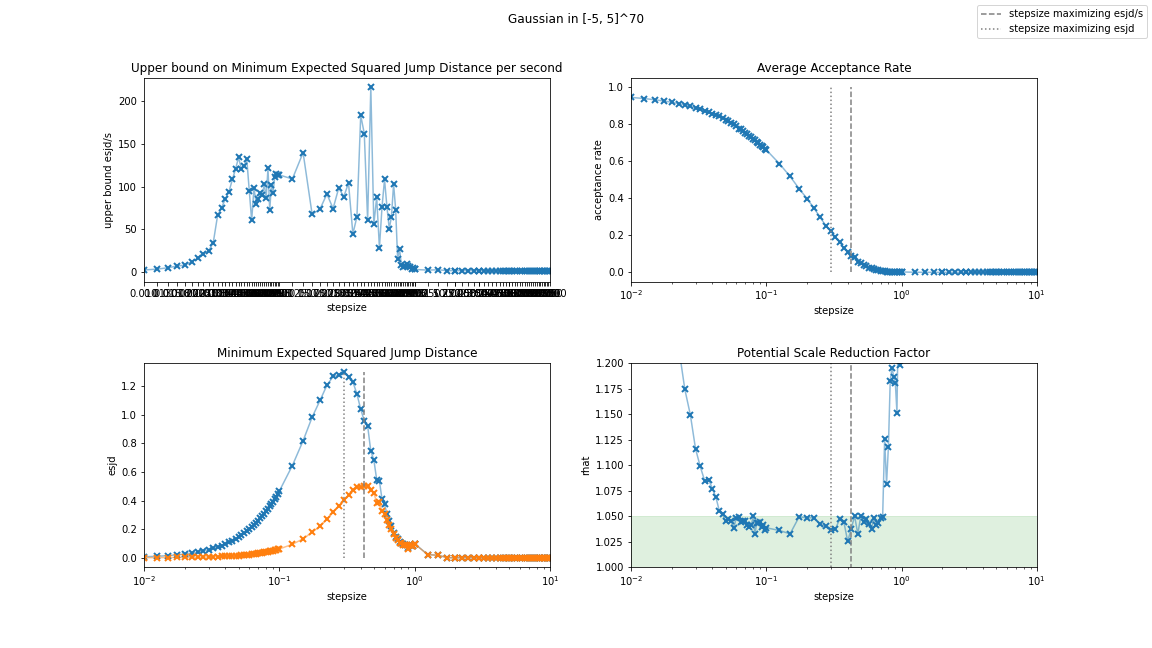
\includegraphics[width=0.7\textwidth]{imgs/bound-5-dim-70-Gaussian-results.png}
\end{frame}

\begin{frame}[t]
    \frametitle{Optimal acceptance rates}
    \begin{itemize}
    \item {\color{orange} Orange } upper bound on the ESJD/s
    \end{itemize}
    \centering
    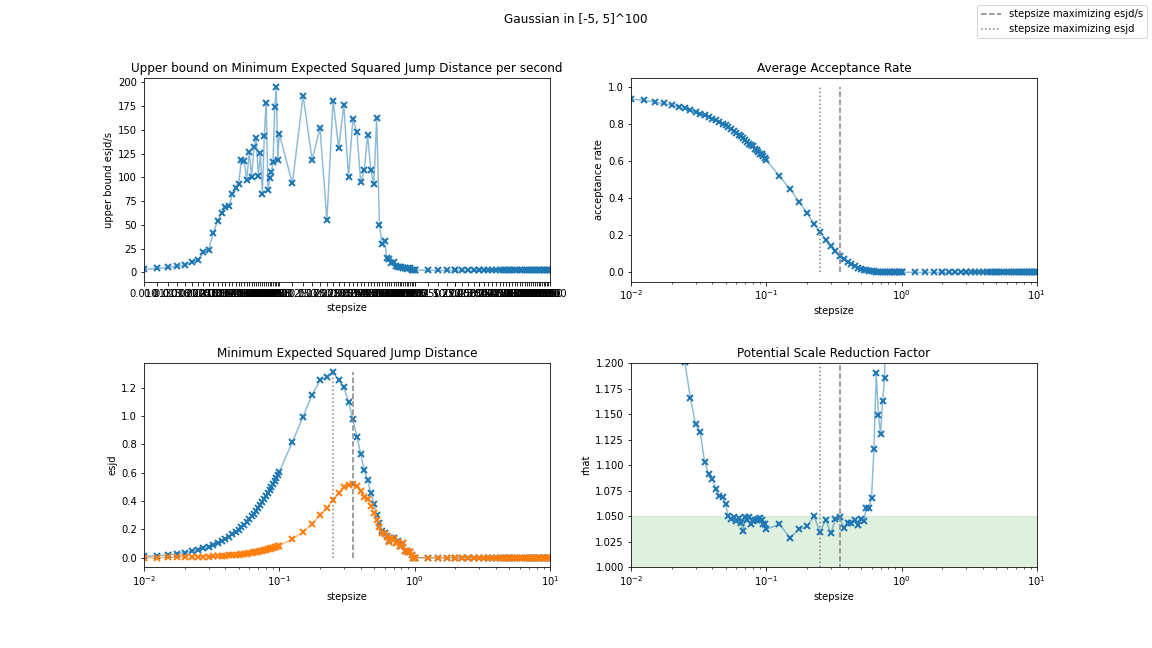
\includegraphics[width=0.7\textwidth]{imgs/bound-5-dim-100-Gaussian-results.png}
\end{frame}

\begin{frame}[t]
    \frametitle{Optimal acceptance rates}
    \begin{itemize}
    \item Optimal acceptance rate per dimension
    \end{itemize}
    \centering
    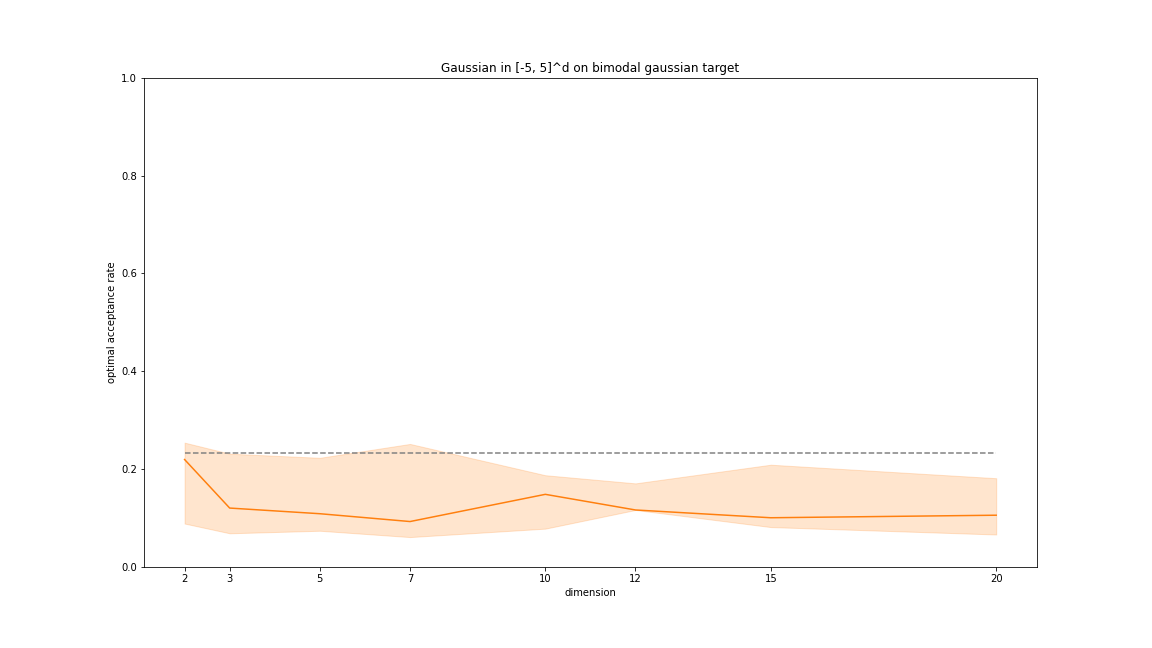
\includegraphics[width=0.7\textwidth]{imgs/bound-5-Gaussian.png}
\end{frame}

\begin{frame}[c]
    \frametitle{Optimal acceptance rates}
    \begin{itemize}
        \item Justifies two things:
        \begin{itemize}
            \item Use ESJD instead of ESS, as it is more robust, cheaper and seems like a good estimator
            \item Tuning to theoretically optimal 0.234 does not hold, if we consider time costs \& costly simulations
        \end{itemize}
        \item Motivates: Offline tuning of the stepsize using ESJD
    \end{itemize}
\end{frame}

\begin{frame}[t]
    \frametitle{Offline tuning using ESJD}
    \begin{columns}
        \begin{column}{0.4\textwidth}
            \centering
            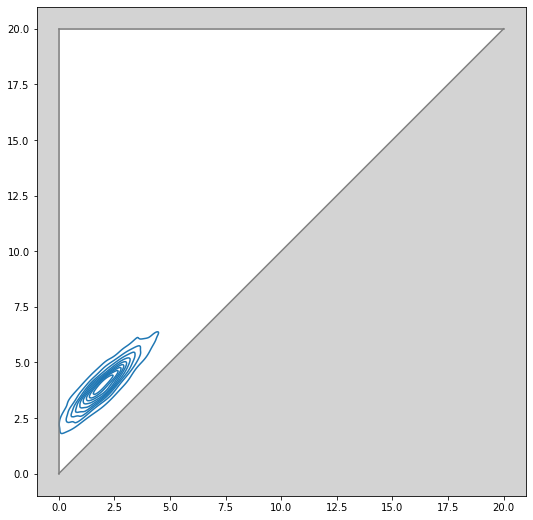
\includegraphics[width=\textwidth]{imgs/time-inhomogeneous}
        \end{column}
        \begin{column}{0.5\textwidth}
            \begin{itemize}
                \item First Approach: 
                \begin{itemize}
                    \item Objective function draws $N$ samples using stepsize $s$ and compute ESJD.
                    \item Plug objective function in general-purpose optimizer
                \end{itemize}
                \item Issue: Objective function is time-inhomogeneous and/or noisy
                \begin{itemize}
                    \item Low probability starting point errorneously favors large step sizes
                \end{itemize}
                \item[]
                \item[$\to$] Possibly calls for \emph{Bayesian optimization} approaches?
                \item[$\to$] Log-uniform sampling of stepsize parameters?
            \end{itemize}
        \end{column}
    \end{columns}
\end{frame}

\begin{frame}[c]
    \frametitle{Starting point selection}
    \begin{itemize}
        \item We want to optimize step size for the "interesting bits", so we first need to get there
        \item[$\to$] Typical warm start procedure is \emph{burn in}
        \item[]
        \item Charles Geyer: \\
            {\centering
            \emph{"Any point you don't mind having in a sample is a good starting point."}\footnote{http://users.stat.umn.edu/~geyer/mcmc/burn.html}
        } \\[1mm]
        \item[$\to$] Use \emph{maximum a posteriori}/\emph{maximum likelihood} estimator by first optimizing the target distribution
    \end{itemize}
    \centering
\end{frame}

\begin{frame}[t]
    \frametitle{Proposal Preconditioning: Polytope Rounding}
	\begin{columns}
        \begin{column}{0.3\textwidth}
            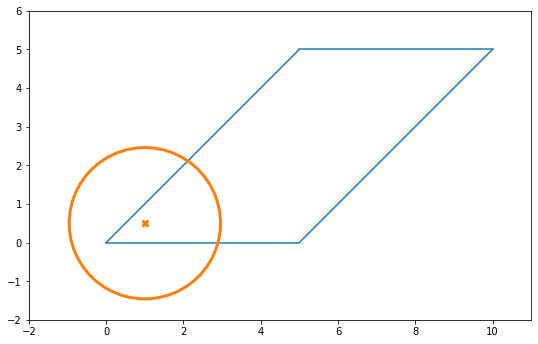
\includegraphics[width=\textwidth]{imgs/no-preconditioning.png}
            Polytope:
            \[
                \mathcal{P} = \{ x : Ax \leq b \}
            \]
            Proposal:
            \[
                x'_{n} = x_n + z, \quad z \sim \mathcal{N}(0,I)
            \]
        \end{column}
        \begin{column}{0.3\textwidth}
            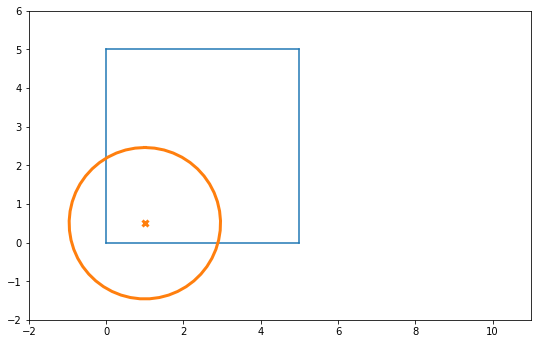
\includegraphics[width=\textwidth]{imgs/proposal-preconditioning.png}
            Polytope:
            \[
                \mathcal{P} = \{ x : ATx \leq b \}
            \]
            Proposal:
            \[
                x'_{n} = x_n + z, \quad z \sim \mathcal{N}(0,I)
            \]
        \end{column}
        \begin{column}{0.3\textwidth}
            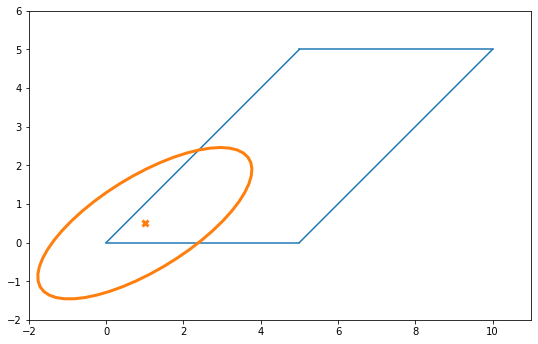
\includegraphics[width=\textwidth]{imgs/polytope-preconditioning.png}
            Polytope:
            \[
                \mathcal{P} = \{ y : Ay \leq b \}, \quad y = Tx
            \]
            Proposal:
            \begin{align*}
                y'_{n} = y_n + Tz, \quad z \sim \mathcal{N}(0,I)
            \end{align*}
        \end{column}
	\end{columns}
\end{frame}

\begin{frame}[t]
    \frametitle{Proposal Preconditioning: Dikin Ellipsoid and/or Fisher Matrix}
    \begin{columns}
    \begin{column}{0.45\textwidth}
        \begin{center}
        %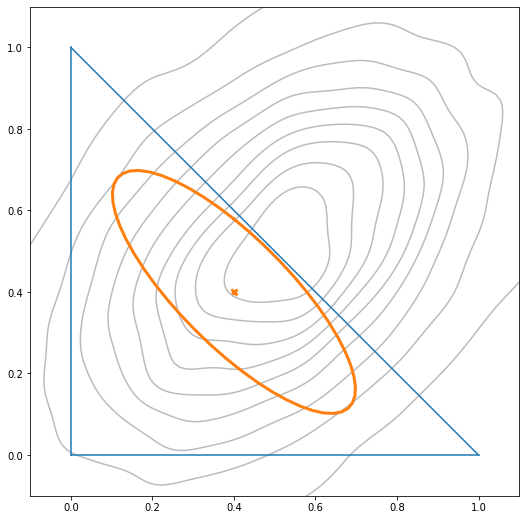
\includegraphics[width=0.7\textwidth]{imgs/dikin-ellipsoid}
        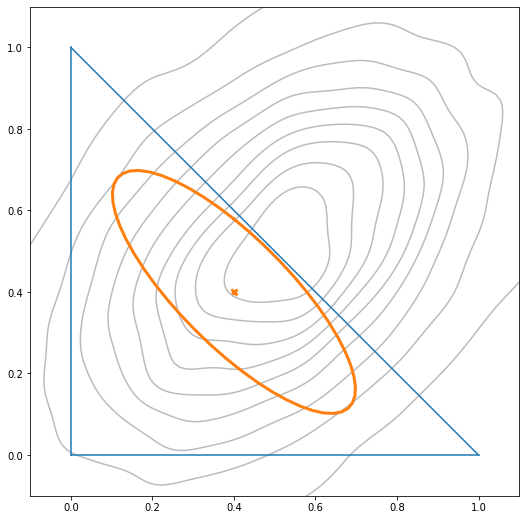
\includegraphics[width=\textwidth]{imgs/dikin-ellipsoid}
        \end{center}
    \end{column}
    \begin{column}{0.45\textwidth}
        Dikin Walk \cite{Kannan2012}:
        \[
            x'_{n} = x_n + \frac{r}{\sqrt{d}}D^{-1/2}z, \quad z \sim \mathcal{N}(0,I)
        \]
        with
        \[
            D = \sum_i \frac{a_i a_i^\top}{(b_i - a_i^\top x)^2} 
        \]
    \end{column}
    \end{columns}
\end{frame}

\begin{frame}[t]
    \frametitle{Proposal Preconditioning: Dikin Ellipsoid and/or Fisher Matrix}
    \begin{columns}
    \begin{column}{0.45\textwidth}
        \begin{center}
        %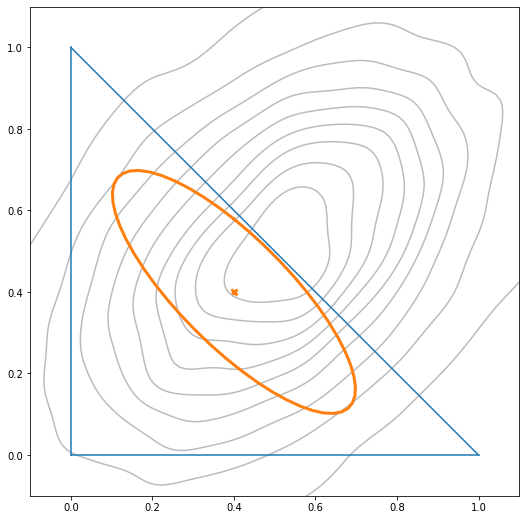
\includegraphics[width=0.7\textwidth]{imgs/dikin-ellipsoid}
        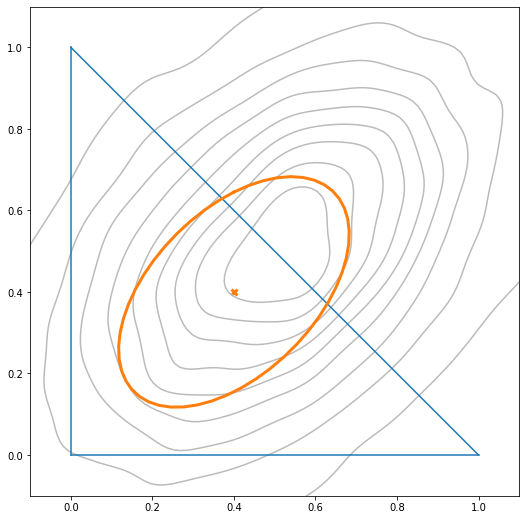
\includegraphics[width=\textwidth]{imgs/fisher-ellipsoid.png}
        \end{center}
    \end{column}
    \begin{column}{0.45\textwidth}
        CSmMALA (s=1) without drift \cite{Theorell2019}:
        \[
            x'_{n} = x_n + rF^{-1/2}z, \quad z \sim \mathcal{N}(0,I)
        \]
        with
        \[
            F = -\mathbb{E}\Big[\pdv[2]{x}\log \mathcal{L}(d|x)\Big| x \Big], 
        \]
        with $\mathcal{L}$ being the likelihood function
    \end{column}
    \end{columns}
\end{frame}

\begin{frame}[t]
    \frametitle{Proposal Preconditioning: Dikin Ellipsoid and/or Fisher Matrix}
    \begin{columns}
    \begin{column}{0.45\textwidth}
        \begin{center}
        %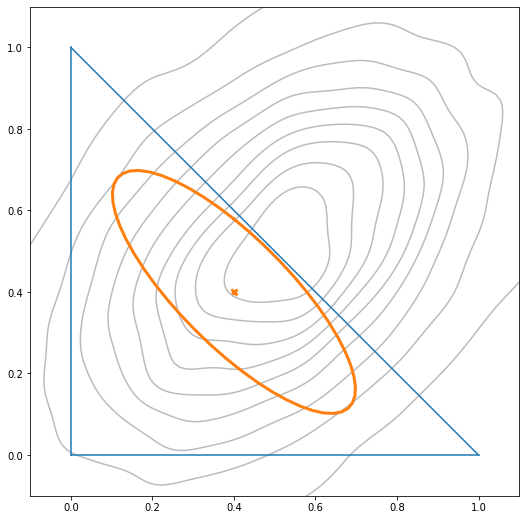
\includegraphics[width=0.7\textwidth]{imgs/dikin-ellipsoid}
        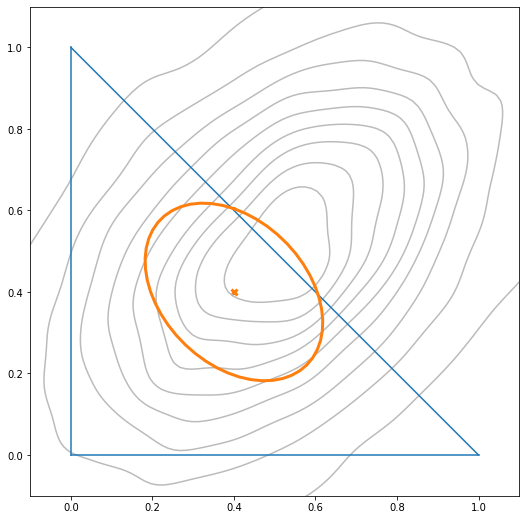
\includegraphics[width=\textwidth]{imgs/fisher-dikin-ellipsoid.png}
        \end{center}
    \end{column}
    \begin{column}{0.45\textwidth}
        CSmMALA (s=0.5) without drift \cite{Theorell2019}:
        \[
            x'_{n} = x_n + rG^{-1/2}z, \quad z \sim \mathcal{N}(0,I)
        \]
        with
        \[
            G = sF + (1-s)D    
        \]
        with $\mathcal{L}$ being the likelihood function
    \end{column}
    \end{columns}
\end{frame}

\begin{frame}[c]
    \frametitle{Proposal Preconditioning: Dikin Ellipsoid and/or Fisher Matrix}
    \begin{itemize}
        \item CSmMALA(s=0.5) 40 times higher ESS as the second best algorithm for a Gaussian target \cite{Theorell2019}
        \item CSmMALA takes two orders of magnitude more time for real \Ciso data
        \item[$\to$] \textbf{Gradients of \Ciso too expensive}
    \end{itemize}
\end{frame}

\begin{frame}[c]
    \frametitle{Local Approximations and Gradient Esimation}
    \begin{itemize}
        \item Idea: Use local approximations of the target function, that are easy to evaluate
        \item \emph{How do we construct such approximations?}
        \item[$\to$] Conrad et al. have the answer! \cite{Conrad2016}
    \end{itemize}
\end{frame}

\begin{frame}[c]
    \frametitle{Local Approximations and Gradient Esimation}
    \begin{itemize}
        \item Maintain set $\mathcal{S}$ of samples and their values, independently from chain samples
        \item Choose $N_L = \sqrt{d} (d + 1)$ or $N_Q= \sqrt{d} (d + 1)(d + 2) / 2$ points for linear or quadratic model respectively which are nearest to current state
        \item Fit model and cross-validate it on the $N$ samples
        \item If error threshold is exceeded, add new point to $\mathcal{S}$
        \item[]
        \item Conrad et al. \cite{Conrad2016} replace exact target function with approximate one, thus sample the "wrong" distribution
        \item We only want to estimate the local gradient by using the fitted model's gradient
        \item Try updating the quadratic model with less points than $N_Q$ by using least Frobenius norm update \cite{Powell2004}
    \end{itemize}
\end{frame}

\begin{frame}[c]
    \frametitle{What to do with the Gradient Esimate?}
    \begin{itemize}
        \item Accelerate CSmMALA
        \item Precondition Hit \& Run algorithm with Fisher information estimate
    \end{itemize}
\end{frame}

\begin{frame}[c]
    \frametitle{What to do with the Gradient Esimate?}
    \begin{itemize}
        \item Accelerate CSmMALA
        \item \textbf{Precondition Hit \& Run algorithm with Fisher information estimate}
    \end{itemize}
\end{frame}

\begin{frame}[c]
    \frametitle{Fisher-preconditioned Hit \& Run?}
    \begin{itemize}
        \item CSmMALA takes convex combination of Dikin \& Fisher information to remain inside polytope \& adapt to target function
        \item Hit \& Run is guaranteed to remain inside polytope! 
        \item[$\to$] Precondition it with Fisher information matrix to adapt to target function
        \item[]
        \item Hit \& Run works best in rounded polytopes
        \item[$\to$] \textbf{Pitfall:} Take care to \emph{round} target function, i.e. evaluate it at the correct position
    \end{itemize}
\end{frame}

\begin{frame}[c]
    \frametitle{Roadmap}
    \begin{itemize}
        {\color{lgray}
            \item Experimentally assess optimal acceptance rates for model problems. Do theoretical results hold?
        }
        \item Offline stepsize tuning starting from MAP estimate
        \item Local approximation and gradient estimates for cheap preconditioning
    \end{itemize}
    \bigskip
    Postponed:
    { \tiny
    \begin{itemize}
	\item How do non-identifiable dimensions affect the optimal acceptance rate and convergence?
	\item Combine Adaptive Metropolis with polytope samplers
	\item Is Adaptive Metropolis able to approximate optimal acceptances rates? 
	\item Does Adaptive Metropolis work with non-identifiable dimensions?
	\item What other approaches exist there? Active subspaces \cite{Constantine_2016}
    \end{itemize}
    }
\end{frame}

\begin{frame}[c]{}
    \centering
    \Huge \emph{Thanks!}
\end{frame}



\end{document}
